\documentclass[a4paper]{oblivoir}

\title{쟤료공학개론 과제4}
\author{2018-12432, Electrical and Computer Engineering department, ParkJeonghyun}
\date{10/22/2023}

\newcommand{\be}{\begin{equation}}
\newcommand{\ee}{\end{equation}}

\usepackage{fapapersize}
\usepackage{amsmath}
\usepackage{MnSymbol}
\usepackage{wasysym}
\usepackage{graphicx}
\usepackage{caption}
\usepackage{subfig}
\usepackage{hyperref}
\usepackage{cite}
\usepackage{dtk-logos}
\usepackage{physics}
\usepackage{tikz}
\usetikzlibrary{decorations.markings, positioning}
\usepackage{dtk-logos}
\usepackage{fancyvrb}
\usepackage{array} 
\usepackage{chemformula}

\usefapapersize{ 210mm, 297mm, 15mm, 15mm, 15mm, 15mm}
\DeclareGraphicsExtensions{.pdf, .png, .jpg}

\renewcommand{\figurename}{Figure}

\begin{document}

\maketitle
\section{Problem 1}
\subsection{a}
\begin{align}
	F &= \frac{dE}{dr}\\
	&=\frac{A}{r^{2}} - \frac{nB}{r^{n+1}}
\end{align}

\subsection{b}
\begin{align}
	\frac{dF}{dr} &= -\frac{2A}{r^{3}} + \frac{n(n+1)B}{r^{n+2}}
\end{align}

\subsection{c}
\begin{align}
	\frac{A}{r^{2}} - \frac{nB}{r^{n+1}} = 0
\end{align}
따라서
\begin{align}
	r_{0} &= \left( \frac{nB}{A}\right)^{\frac{1}{n-1}}
\end{align}

\subsection{d}
\begin{align}
	\frac{dF}{dr} &= -\frac{2A}{r_{0}^{3}} + \frac{n(n+1)B}{r_{0}^{n+2}}\\
	&= \frac{n(n-1)B}{r_{0}^{n+2}}\\
	&= n(n-1)B\left( \frac{A}{nB}\right)^{\frac{n+2}{n-1}}
\end{align}

\section{Problem 2}
\subsection{a}
\begin{align}
	\sigma &= E\epsilon\\
	&= E\frac{\Delta l}{l}
\end{align}
따라서
\begin{align}
	\Delta l &= \frac{Fl}{AE}\\
	&= \frac{48900 \times 4 \times 250 \times 10^{-3}}{\pi(15.2\times 10^{-3})^{2}\times 207\times10^{9}} m\\
	&= 3.25 \times 10^{-4}m
\end{align}

\subsection{b}
\begin{align}
	\gamma &= - \frac{\Delta d / d}{\Delta l / l}
\end{align}
따라서
\begin{align}
	\Delta d &= - \gamma \frac{d\Delta l}{ l}\\
	&= - 0.30 \frac{15.2\times 10^{-3}\times 3.25 \times 10^{-4}}{250\times10^{-3}}m\\
	&= -5.93 \times 10^{-6}m
\end{align}

\section{Problem 3}
\subsection{a}
\begin{align}
	E &= \frac{d\sigma}{d\epsilon}\\
	&= \frac{1000\times10^{6}}{0.005} Pa\\
	&= 200 GPa
\end{align}

\subsection{b}
Proportional limit은 $\sigma = E \epsilon$의 linearity가 만족하지 않는 stress이다. 따라서 $1400MPa$

\subsection{c}
Fig.\ref{fig:p3c}에서 알 수 있듯 yield strength at a strain offset of 0.002는 약 $1600MPa$이다.
\begin{figure}[h]
    \centering
    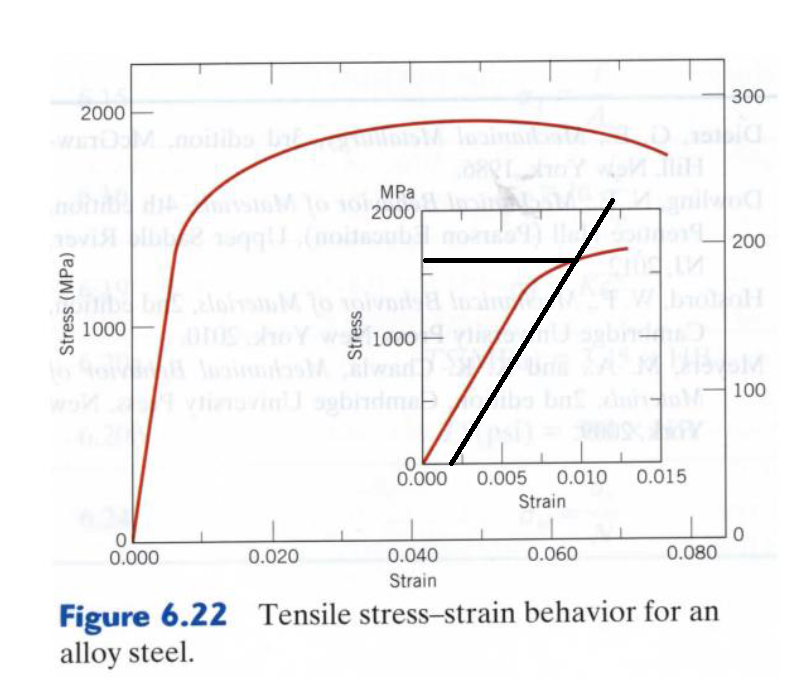
\includegraphics[width=0.5\linewidth]{p3c.png}
    \caption{\label{fig:p3c} yield strength 그래프}
\end{figure}

\subsection{d}
Fig.\ref{fig:p3d}에서 알 수 있듯 tensile strength는 약 $1950MPa$이다.
\begin{figure}[h]
    \centering
    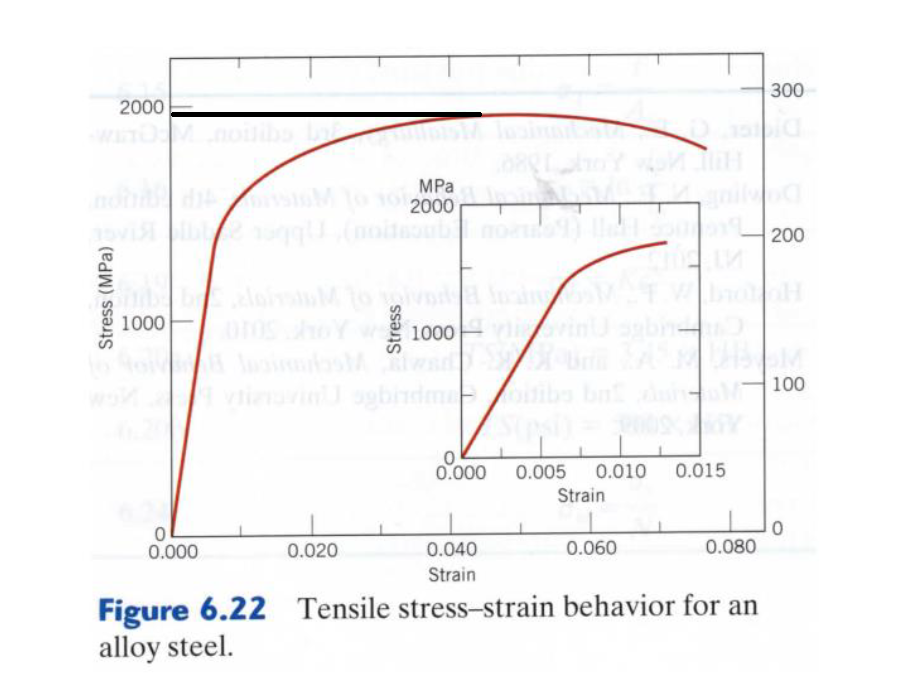
\includegraphics[width=0.5\linewidth]{p3d.png}
    \caption{\label{fig:p3d} tensile strength 그래프}
\end{figure}

\section{Problem 4}
\subsection{a}
Engineering stress와 true stress는 각각 아래와 같이 나타난다.
\begin{align}
	\sigma &= \frac{F}{A_{0}}\\
	\sigma_{T} &= \frac{F}{A_{i}}\\
	&= \frac{F}{A_{0}}\frac{l_{i}}{l_{0}}\\
	&= \sigma (1+\epsilon)
\end{align}

Engineering strain과 true strain은 각각 아래의 관계를 만족한다.
\begin{align}
	\epsilon &= \frac{l_{i}}{l_{0}}-1\\
	\epsilon_{T} &= \int_{l_{0}}^{l_{i}}\frac{dl}{l}\\
	&= \ln{\frac{l_{i}}{l_{0}}}\\
	&= \ln{(1+\epsilon)}
\end{align}

\end{document}